\documentclass{article}

\usepackage{arxiv}

\usepackage[utf8]{inputenc} % allow utf-8 input
\usepackage[T1]{fontenc}    % use 8-bit T1 fonts
\usepackage{lmodern}        % https://github.com/rstudio/rticles/issues/343
\usepackage{hyperref}       % hyperlinks
\usepackage{url}            % simple URL typesetting
\usepackage{booktabs}       % professional-quality tables
\usepackage{amsfonts}       % blackboard math symbols
\usepackage{nicefrac}       % compact symbols for 1/2, etc.
\usepackage{microtype}      % microtypography
\usepackage{graphicx}

\title{Current status and prospects of R-packages for the design of
experiments}

\author{
    Emi Tanaka
    \thanks{emitanaka.org}
   \\
    Department of Econometrics and Business Statistics \\
    Monash University \\
  Clayton, VIC 3800 \\
  \texttt{\href{mailto:emi.tanaka@monash.edu}{\nolinkurl{emi.tanaka@monash.edu}}} \\
   \And
    Dewi Amaliah
   \\
    Department of Econometrics and Business Statistics \\
    Monash University \\
  Clayton, VIC 3800 \\
  \texttt{} \\
  }


% tightlist command for lists without linebreak
\providecommand{\tightlist}{%
  \setlength{\itemsep}{0pt}\setlength{\parskip}{0pt}}


% Pandoc citation processing
\newlength{\cslhangindent}
\setlength{\cslhangindent}{1.5em}
\newlength{\csllabelwidth}
\setlength{\csllabelwidth}{3em}
\newlength{\cslentryspacingunit} % times entry-spacing
\setlength{\cslentryspacingunit}{\parskip}
% for Pandoc 2.8 to 2.10.1
\newenvironment{cslreferences}%
  {}%
  {\par}
% For Pandoc 2.11+
\newenvironment{CSLReferences}[2] % #1 hanging-ident, #2 entry spacing
 {% don't indent paragraphs
  \setlength{\parindent}{0pt}
  % turn on hanging indent if param 1 is 1
  \ifodd #1
  \let\oldpar\par
  \def\par{\hangindent=\cslhangindent\oldpar}
  \fi
  % set entry spacing
  \setlength{\parskip}{#2\cslentryspacingunit}
 }%
 {}
\usepackage{calc}
\newcommand{\CSLBlock}[1]{#1\hfill\break}
\newcommand{\CSLLeftMargin}[1]{\parbox[t]{\csllabelwidth}{#1}}
\newcommand{\CSLRightInline}[1]{\parbox[t]{\linewidth - \csllabelwidth}{#1}\break}
\newcommand{\CSLIndent}[1]{\hspace{\cslhangindent}#1}

\usepackage{colortbl}
\usepackage{xcolor}
\usepackage{hyperref}
\usepackage[utf8]{inputenc}
\def\tightlist{}

\begin{document}
\maketitle


\begin{abstract}
Re-running an experiment is generally costly and in some cases
impossible due to limited resources, so the design of an experiment
plays a critical role in increasing the quality of experimental data. In
this article we describe the current state of the R-packages for the
design of experiments through exploratory data analysis of package
downloads, package metadata, and comparison of characteristics with
other topics. We discuss also the software design of widely utilised R
packages in the field of experimental design and conclude with
discussion of some future prospects for the field.
\end{abstract}


\hypertarget{introduction}{%
\section{Introduction}\label{introduction}}

The critical role of data collection is well captured in the expression
``garbage in, garbage out'' -- in other words, if the collected data is
rubbish then no analysis, however complex it may be, can make something
out of it. Methods for data collection can be dichotomised by the type
of data collected -- namely, experimental or observational -- or
alternatively, categorised as experimental design (including
quasi-experimental design) or survey design. This dichotomisation, to a
great extent, is seen in the
\href{https://cran.r-project.org/web/views/}{CRAN task views} (a
volunteered maintained list of R-packages by topic) where R-packages in
experimental design are in ctv\{ExperimentalDesign\} and R-packages in
survey designs are in ctv\{OfficialStatistics\}. Experimental designs
exclusively center on the collection of experimental data where many of
the experimental factors tend to be in the control of the experimenter.
A subset of experimental designs are segregated into
ctv\{ClinicalTrials\}, where the focus is on clinical trials with
primary interest in sample size calculations. This paper focuses on the
packages in ctv\{ExperimentalDesign\}, henceforth referred to as ``DoE
packages''.

In the CRAN task view of ctv\{ExperimentalDesign\}, there are 114 R
packages for experimental design and analysis of data from experiments.
The sheer quantity and variation of experimental designs in the
R-packages are arguably unmatched with any other programming languages,
e.g.~in Python (Rossum 1995), only a handful of libraries that generate
design of experiment exist (namely \texttt{pyDOE}, \texttt{pyDOE2},
\texttt{dexpy}, \texttt{experimenter} and \texttt{GPdoemd}) with limited
type of designs. Thus, the study of DoE packages can be revealing into
the current status of the field of experimental design.

The paper is organised as follows. Section @ref(data) briefly describes
the data source used for the analysis in Section @ref(eda); Section
@ref(eda) presents some insights into the state of the current DoE
packages by exploratory data analysis of package download data, text
descriptions and comparisons with other CRAN task views; Section
@ref(design) discuss the interface designs of DoE packages, and we
conclude with a discussion in Section @ref(discussion) of future
prospects.

\hypertarget{data}{%
\section{Data}\label{data}}

To study the DoE packages, we analyse data using three sources of data
as described next.

\hypertarget{rstudio-cran-download-logs}{%
\subsection{RStudio CRAN download
logs}\label{rstudio-cran-download-logs}}

The Comprehensive R Archive Network (CRAN) is a network of servers
located across the world that store mirrored versions of R and
R-packages. The most popular network is the RStudio mirror (the default
server for those that use the RStudio IDE). The RStudio mirror is also
the only server that provides a comprehensive daily download logs of R
and R-packages since October 2012. The summary data can be easily
accessed with the \texttt{cranlogs} package (Csárdi 2019). This paper
uses the data from the beginning of 2013 to end of 2021 (a total of 9
years) for the DoE packages.

\hypertarget{package-descriptions}{%
\subsection{Package descriptions}\label{package-descriptions}}

All CRAN packages have a title, description, package connections
(suggests, dependency and imports) and other meta-information in the
DESCRIPTION file. We use the text data from the title and description
(as accessed in 2022-05-23) in Section @ref(topics).

\hypertarget{cran-task-views}{%
\subsection{CRAN task views}\label{cran-task-views}}

The list of packages in each CRAN task views (as of 2022-05-25) are used
to contrast the characteristics of DoE packages in Section @ref(silo).

\hypertarget{eda}{%
\section{Explorative data analysis}\label{eda}}

All results presented are derived from exploratory data analysis of
observational data; consequently, all interpretations are somewhat
speculative and may not be indicative of the true state of the field of
experimental design. In particular, any analysis over time are
confounded by the fact that the nature of users and package management
have also changed over the years. It should be noted that some DoE
packages may have been archived or removed from the task view over the
years so any cross-sectional analysis presented may not reflect the set
of all DoE packages at that particular time period (although we assume
such incidences are low).

A subset of DoE packages is not primarily about design of experiments
but about the analysis of experimental data. A complete delineation of
these packages is difficult as many have some functions that can aid
decisions or constructions of experimental designs (and any
categorisation is prone to our subjective bias) so we opted not to
remove any DoE packages in the analysis.

\hypertarget{popular}{%
\subsection{Small, but diverse, set of packages are sufficient for most
designs}\label{popular}}

There have been at least 50 DoE packages since 2013 but most of the
downloads are concentrated in just a handful of packages. For example,
Figure @ref(fig:plot-lorenz) shows a Lorenz curve (Lorenz 1905) for the
total package downloads in 2021 of 113 DoE packages (first released
prior to 2021); we can see from Figure @ref(fig:plot-lorenz) that bottom
90\% of DoE packages (in terms of total download count in 2021) only
share about 30\% of total downloads across all DoE packages -- in
another words, 70\% of the total downloads are due to 11 packages (10\%
of the DoE packages).

\begin{figure}[htbp]

{\centering 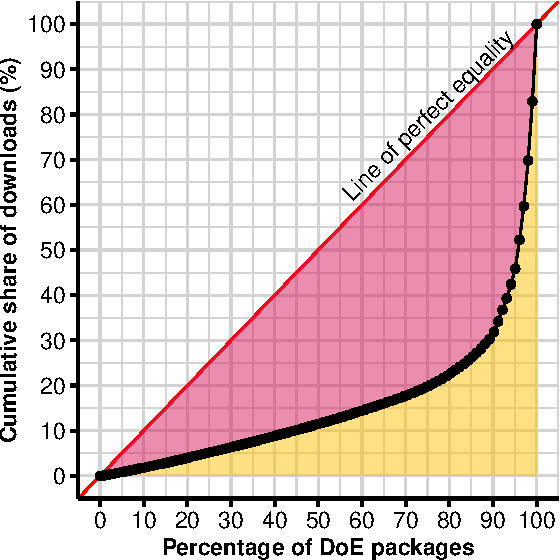
\includegraphics{figures/plot-lorenz-1} 

}

\caption{Lorenz curve of the total download count for DoE packages in 2021. The red line corresponds to the line of perfect equality.}\label{fig:plot-lorenz}
\end{figure}

If we consider package downloads as a measure of ``wealth'', then we can
consider using the Gini index (Gini 1921) as a measure of download
inequality across packages. The ratio of the red region over the total
colored regions in Figure @ref(fig:plot-lorenz) corresponds to the Gini
index for 2021. A Gini index of 0\% indicates equality in downloads
across packages while a value of 100\% indicates maximal inequality (all
downloads are due to one package). In Figure @ref(fig:download-share),
we see that the distributions of the downloads each year have a heavy
right tail with the Gini index ranging from 32.5\% to 68.3\% across the
years 2013 to 2021, indicating that there is a high level of inequality
of downloads across packages, particularly with more pronounced
inequality in the last 5 years.

\begin{figure}[htbp]

{\centering 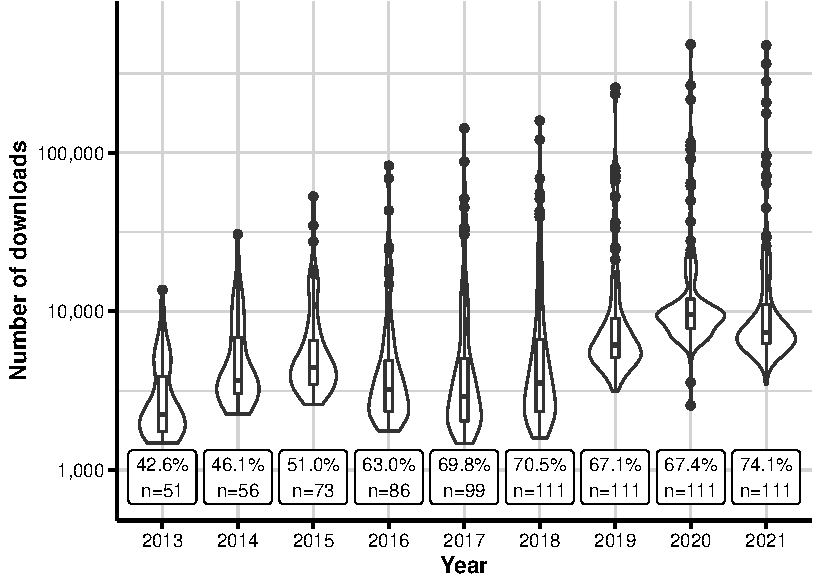
\includegraphics{figures/download-share-1} 

}

\caption{The distribution of the number of downloads for each DoE package by year. Packages were removed in any year if it was released in that year or later so that each download count is for the full year. The label on the bottom of the plot shows the Gini index for downloads and the number of packages with full year of download count in the corresponding year. In the last 5 years, the Gini index is consistent above 60\% each year indicating that most downloads are due to a relatively small number of packages.}\label{fig:download-share}
\end{figure}

While in absolute terms the Gini index is high for
ctv\{ExperimentalDesign\}, the inequality is not as severe as other CRAN
task views as shown in Figure @ref(fig:fig-gini-all-ctvs). We can see in
Figure @ref(fig:fig-gini-all-ctvs) that the Gini index is generally
increasing for DoE packages (as is generally the case for other CRAN
task views as shown in Figure S1 in the Supplementary Materials).

\begin{figure}[htbp]

{\centering 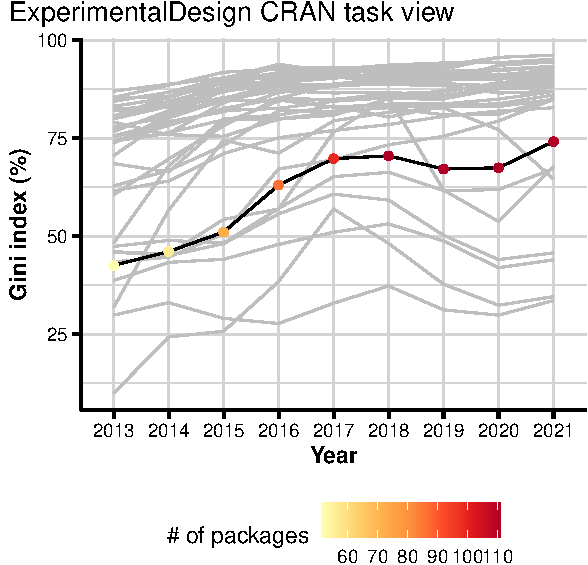
\includegraphics{figures/fig-gini-all-ctvs-1} 

}

\caption{The points show the Gini index of the download counts by year facetted by CRAN task view with the color showing the number of packages. The grey line shows the distribution of the Gini index across years for all other CRAN task views. The facets are ordered by increasing value of the Gini index in 2021.}\label{fig:fig-gini-all-ctvs}
\end{figure}

From Figures @ref(fig:download-share) and @ref(fig:fig-gini-all-ctvs),
we could draw some indicative states of the field of experimental
designs with possible counterfactual interpretations:

\begin{itemize}
\tightlist
\item
  The increase in the number of packages that are not highly downloaded
  may mean that \textbf{\emph{there are more packages to construct niche
  experimental designs}}. Some examples of these packages include
  \texttt{qtlDesign}, \texttt{PwrGSD} and \texttt{Crossover} made for
  QTL experiments, group sequential designs and crossover trials,
  respectively. These packages would naturally have a smaller number of
  potential users. Counterfactual to this, the increase could be due to
  other external factors, such as an increase in a number of skilled
  contributors, a change in CRAN policy or management to add packages
  (either to CRAN and/or task view), and/or that new packages are still
  yet to amass users. While there is an argument that low download
  counts are due to the low utility and/or quality of the packages,
  packages in CRAN task views are selected by expert maintainers; thus
  we can reasonably assume that any package listed in CRAN task view are
  of a decent utility and quality.
\item
  If the downloads are reflective of the experimental designs used in
  practice, \textbf{\emph{small set of packages appear to be sufficient
  for most to construct the full set of designs of experiments needed in
  practice}}. Packages of course evolve and the top downloaded packages
  have had regular updates that may have broadened its scope.
\item
  While small subset of DoE packages are most frequently used, none of
  these packages are dominant in the field (judging from comparisons
  with other CRAN task views). This suggests that there are
  \textbf{\emph{diverse approaches to designing experiments}}. This
  observation doesn't take into account other approaches to generating
  experimental designs, like the proprietary GUI software, CycDesignN,
  which may be widely used.
\end{itemize}

\hypertarget{ranking}{%
\subsection{There is a lack of adaptation of new or innovative
designs}\label{ranking}}

We can see in Figure @ref(fig:rank-over-time) that most of the top 10
ranking packages have been in the top 10 for the last 9 years with
\texttt{lhs} steadily climbing up the ranks in the last few years.

\begin{figure}[htbp]

{\centering 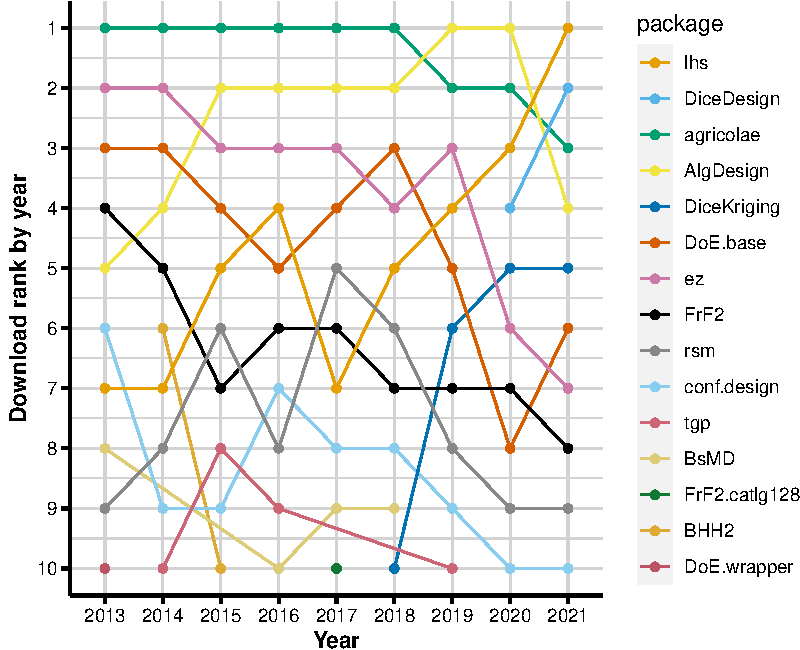
\includegraphics{figures/rank-over-time-1} 

}

\caption{The plot shows the rank of top 10 downloaded packages by year. }\label{fig:rank-over-time}
\end{figure}

Figure @ref(fig:established-packages) shows a moderate negative
correlation between the first release date and the (log of) total
download counts of DoE packages in any given year from 2013 to 2021.
This suggest that in general, a package released earlier are more likely
to be used today (possibly for legacy reasons or the general inertia for
adoption of new packages). We can also see in Figure
@ref(fig:established-packages) the most downloaded packages were
generally released in 2004 to 2010.

\begin{figure}[htbp]

{\centering 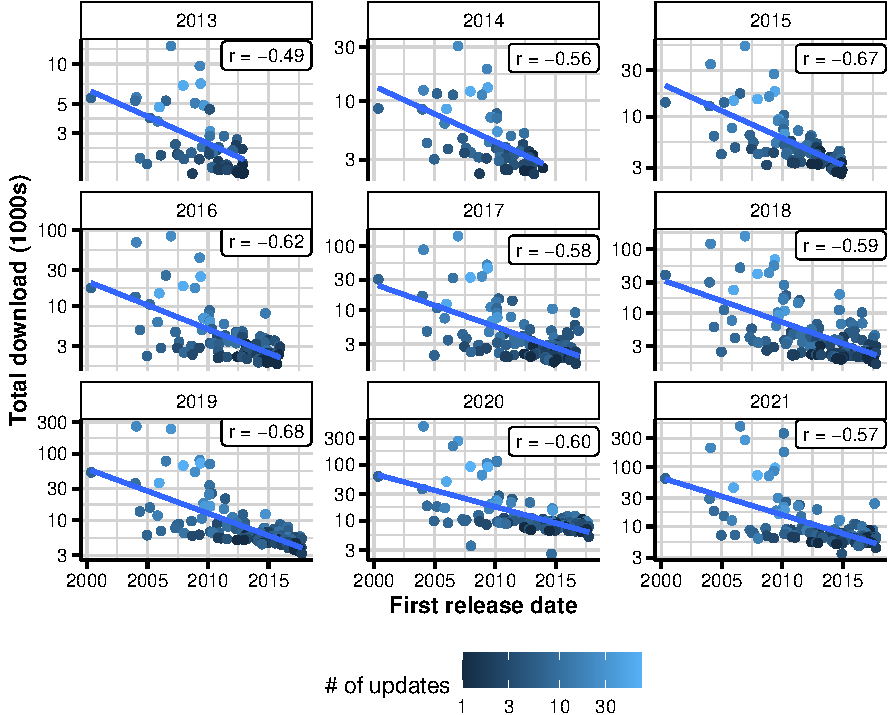
\includegraphics{figures/established-packages-1} 

}

\caption{The above figure shows the total download (in log scale) of a package in the corresponding year against the first release date of the package. The blue line corresponds to the least squares fit of a simple linear regression model. The label in the right-hand upper corner shows the sample correlation coefficient between the first release date and the log, with base 10, of the total download count. The high-leverage point on the far left belongs to `conf.design`, authored by one of the earlier contributors to R.}\label{fig:established-packages}
\end{figure}

The lack of change in the top ranking packages are indicative that there
has been generally little need for new or innovative experimental design
needs for the mass. We do however also see that the the top downloaded
packages generally have more updates so it is possible that the packages
have improved or broadened the scope of its usage.

\hypertarget{topics}{%
\subsection{Computer experiments and optimal designs are of
interest}\label{topics}}

Figure @ref(fig:wordcloud-over-time) shows some common purposes of DoE
packages, based on bigrams in the package title and description. A
bigram is only shown as the frequency of single word was not insightful
and there were not many trigrams common across packages. Not
surprisingly, the bigram ``experimental design'' was the most common.
More interestingly, ``optimal design'' appeared across different
packages (indicated by the size of the word in Figure
@ref(fig:wordcloud-over-time)), and the bigrams ``latin hypercube'' and
``computer experiment'' used across a few packages that are downloaded
frequently (indicated by the color of the word in Figure
@ref(fig:wordcloud-over-time)). Although there exists a separate
ctv\{ClinicalTrials\} task view, the DoE packages clearly include some
packages that are of interest to clinical trials as shown by the size of
the bigram ``clinical trial'' in Figure @ref(fig:wordcloud-over-time).

\begin{figure}[htbp]

{\centering 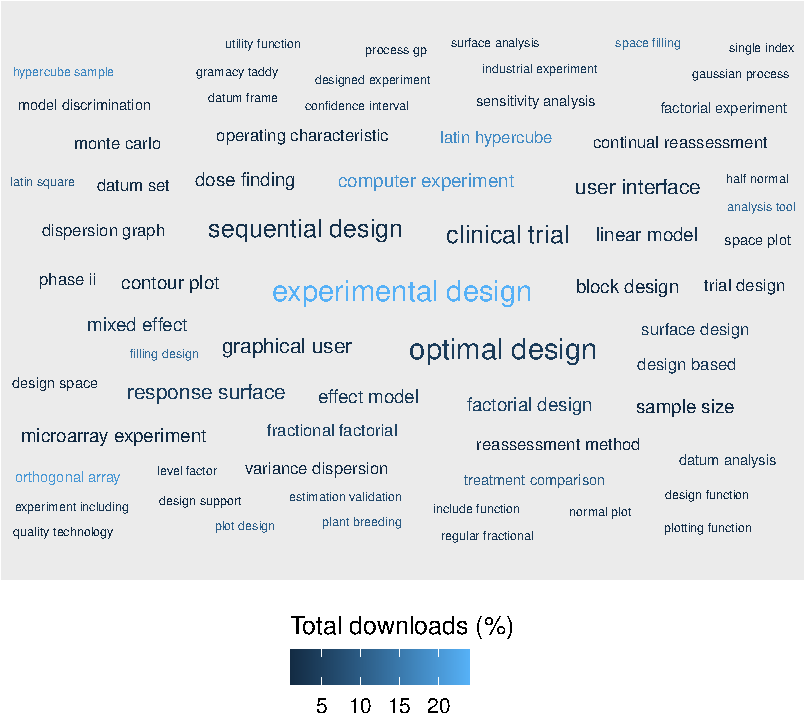
\includegraphics{figures/wordcloud-over-time-1} 

}

\caption{The above figure shows the word cloud of bigrams from the title and descriptions of the CRAN packages. The size shows how often the bigram appears across the DoE packages and the color are relative to the total download count in 2021 of the packages that contain the bigram.}\label{fig:wordcloud-over-time}
\end{figure}

\hypertarget{silo}{%
\subsection{Development of experimental designs occur in
silos}\label{silo}}

Figure @ref(fig:ctv-summ-plot) shows that the ctv\{ExperimentalDesign\}
have the lowest average number of contributors among all CRAN task
views. In addition, we can also see in Figure @ref(fig:ctv-summ-plot)
that the ctv\{ExperimentalDesign\} task view has one of the least
intra-connectivity (the percentage of packages that make use of other
packages within the same task view). The full connection of DoE packages
with other DoE packages is shown in Figure @ref(fig:plot-doe-network).
These observations suggest that the field of experimental design is one
of the least collaborative field and package development generally occur
in silos.

\begin{figure}[htbp]

{\centering 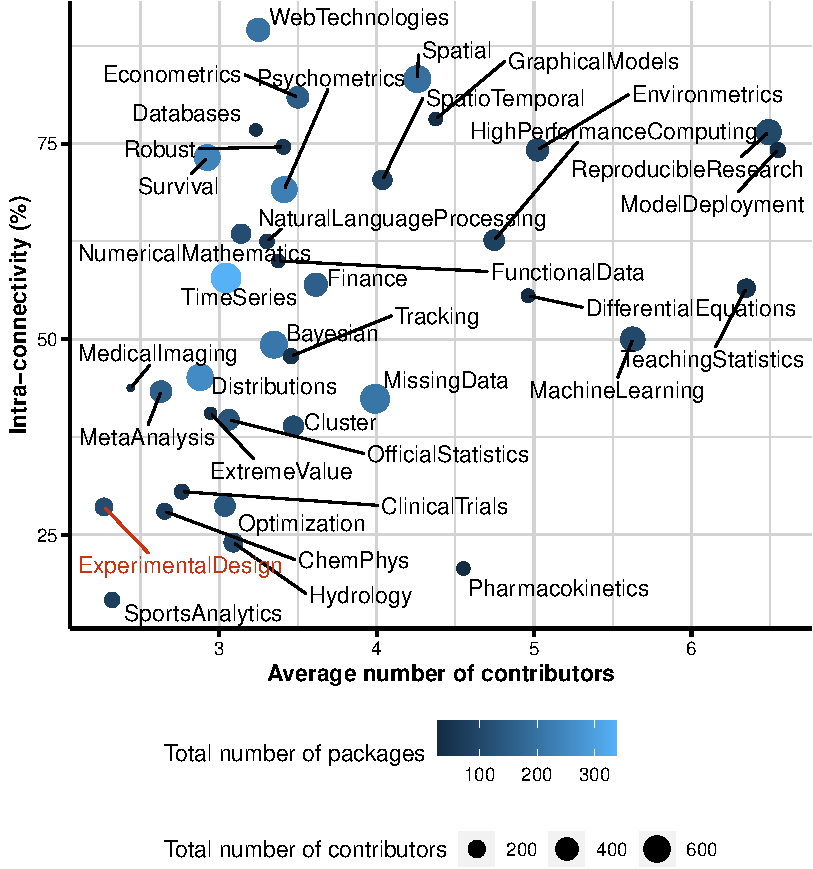
\includegraphics{figures/ctv-summ-plot-1} 

}

\caption{The above figure is a scatterplot of the intra-connectivity (the percentage of packages that depends, suggest or imports at least one other package within the same task view) and the average number of contributors for each CRAN task view. A low intra-connectivity suggests that development within the topic mostly occur in silos whilst high  intra-connectivity suggests that there are more interactions within the topic. The color shows the number of packages, the size of the point corresponds to the total number of contributors, and the text labels show the CRAN task view name.  The label of ExperimentalDesign task view is colored red. The task views in the bottom-left corner are topics that are more indicative of contributors working in silos. The actual numerical values are show in Table S1 in the Supplementary Material.}\label{fig:ctv-summ-plot}
\end{figure}

\begin{figure}[htbp]

{\centering 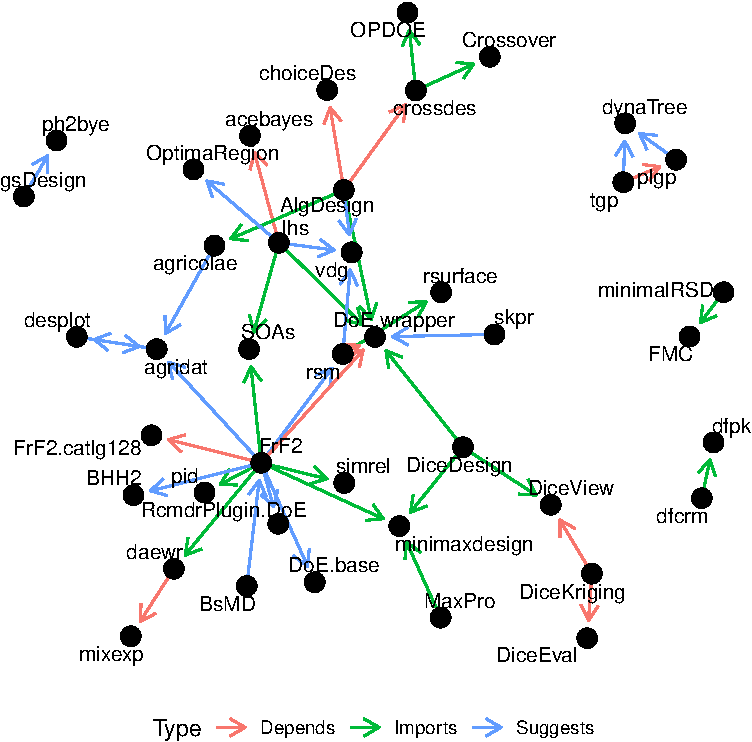
\includegraphics{figures/plot-doe-network-1} 

}

\caption{Package connections (depends, suggests and imports) within the DoE packages. DoE packages that do not depend, suggest or import another DoE package is not shown.}\label{fig:plot-doe-network}
\end{figure}

\hypertarget{design}{%
\section{Interface design}\label{design}}

In software design, there are two interface designs to consider: user
interface (UI) and application programming interface (API). UI is
concerned with the usage of the software by the user, while the API is
concerned with how different programs interact and is predominately of
the interest to the developer. In this section, we discuss these
interface designs broadly, with examples illustrated from the top
downloaded packages (as shown in Figure @ref(fig:rank-over-time)). We
exclude \texttt{ez} and \texttt{DiceKriging} from the discussion as the
former is predominately visualisation of experimental data and latter is
about the analysis of computer experiments in addition to belonging to
the same suite of packages as \texttt{DiceDesign}.

\hypertarget{the-case-of-specialised-designs}{%
\subsection{The case of specialised
designs}\label{the-case-of-specialised-designs}}

In this section, we present some examples the user interface of widely
used specialised designs, namely, computer experiments, factorial
experiments, response surface designs and sequential designs.

Computer experiments, as discussed in Section @ref(topics), which
generally involve space filling designs have been on the rise. The
exemplar for this type of designs are \texttt{lhs} and
\texttt{DiceDesign}. For the \texttt{lhs} package, functions like
\texttt{randomLHS()}, \texttt{optimumLHS()}, and \texttt{maximinLHS()}

Factorial experiments offer a challenge in the construction and
allocation of the treatment factors. This is reflected in a number of
packages that specifically addresses this challenge. These include
\texttt{DoE.base} (Grömping 2018), \texttt{FrF2} (Grömping 2014) for
fractional 2-level factorial designs, \texttt{conf.design} (Venables
2013), \texttt{FrF2.catlg128} (Grömping 2022) and \texttt{BHH2} (Barrios
2016).

Response surface design, as illustrated by \texttt{rsm} (Lenth 2009), is
a type of experiment that involve variables with continuous measures.

Finally, another specialised design is sequential design (also called
adaptive sampling), which is best represented by \texttt{tgp} (Gramacy
and Taddy 2010) -- these require prior information, which are used to
inform the next experimental design. Follow-up experiments, which can
also be classified as a sequential design, is implemented by
\texttt{BsMD} (Barrios 2020).

\hypertarget{the-case-of-menu-functions}{%
\subsection{The case of menu
functions}\label{the-case-of-menu-functions}}

The \texttt{agricolae} package (de Mendiburu 2021) was the most
downloaded DoE packages in 2013 to 2018 (Figure
@ref(fig:rank-over-time)) and possibly prior to 2013 (data unavailable).
This package is the prime example of constructing designs based on menu
functions, e.g.~\texttt{design.crd()}, \texttt{design.rcbd()} and
\texttt{design.split()} construct a completely randomised design,
randomised complete block design and split-plot design, respectively.
Users typically supply the treatment labels and the number of
replications as argument to these functions.

\hypertarget{the-case-of-general-designs}{%
\subsection{The case of general
designs}\label{the-case-of-general-designs}}

\texttt{AlgDesign} (Wheeler 2022)

\texttt{DoE.wrapper} (Grömping 2020)

\hypertarget{discussion}{%
\section{Discussion}\label{discussion}}

Volunteer maintained -- some experimental design packages may not be
included in the CRAN task view.

\hypertarget{acknowledgement}{%
\section{Acknowledgement}\label{acknowledgement}}

This paper uses the \texttt{targets} framework (Landau 2021) for
reproducibility, \texttt{knitr} (Xie 2015) and \texttt{rmarkdown} (Xie,
Allaire, and Grolemund 2018) for creating reproducible documents,
\texttt{ggplot2} (Wickham 2016) for visualisation and
\texttt{kableExtra} (Zhu 2021) for customising the table. All code to
reproduce this paper is found at
\url{https://github.com/emitanaka/paper-DoE-review}.

\hypertarget{references}{%
\section*{References}\label{references}}
\addcontentsline{toc}{section}{References}

\hypertarget{refs}{}
\begin{CSLReferences}{1}{0}
\leavevmode\vadjust pre{\hypertarget{ref-BHH2}{}}%
Barrios, Ernesto. 2016. \emph{Bhh2: Useful Functions for Box, Hunter and
Hunter II}. \url{https://CRAN.R-project.org/package=BHH2}.

\leavevmode\vadjust pre{\hypertarget{ref-BsMD}{}}%
---------. 2020. \emph{BsMD: Bayes Screening and Model Discrimination}.
\url{https://CRAN.R-project.org/package=BsMD}.

\leavevmode\vadjust pre{\hypertarget{ref-cranlogs}{}}%
Csárdi, Gábor. 2019. \emph{Cranlogs: Download Logs from the 'RStudio'
'CRAN' Mirror}. \url{https://CRAN.R-project.org/package=cranlogs}.

\leavevmode\vadjust pre{\hypertarget{ref-agricolae}{}}%
de Mendiburu, Felipe. 2021. \emph{Agricolae: Statistical Procedures for
Agricultural Research}.
\url{https://CRAN.R-project.org/package=agricolae}.

\leavevmode\vadjust pre{\hypertarget{ref-Gini1921-mf}{}}%
Gini, Corrado. 1921. {``Measurement of Inequality of Incomes.''}
\emph{The Economic Journal} 31 (121): 124--26.
\url{https://doi.org/10.2307/2223319}.

\leavevmode\vadjust pre{\hypertarget{ref-tgp}{}}%
Gramacy, Robert B., and Matthew Taddy. 2010. {``Categorical Inputs,
Sensitivity Analysis, Optimization and Importance Tempering with {tgp}
Version 2, an {R} Package for Treed Gaussian Process Models.''}
\emph{Journal of Statistical Software} 33 (6): 1--48.
\url{https://doi.org/10.18637/jss.v033.i06}.

\leavevmode\vadjust pre{\hypertarget{ref-FrF2}{}}%
Grömping, Ulrike. 2014. {``{R} Package {FrF2} for Creating and Analyzing
Fractional Factorial 2-Level Designs.''} \emph{Journal of Statistical
Software} 56 (1): 1--56. \url{https://www.jstatsoft.org/v56/i01/}.

\leavevmode\vadjust pre{\hypertarget{ref-DoE.base}{}}%
---------. 2018. {``{R} Package {DoE.base} for Factorial Experiments.''}
\emph{Journal of Statistical Software} 85 (5): 1--41.
\url{https://doi.org/10.18637/jss.v085.i05}.

\leavevmode\vadjust pre{\hypertarget{ref-DoE.wrapper}{}}%
---------. 2020. \emph{DoE.wrapper: Wrapper Package for Design of
Experiments Functionality}.
\url{https://CRAN.R-project.org/package=DoE.wrapper}.

\leavevmode\vadjust pre{\hypertarget{ref-FrF2.catlg128}{}}%
---------. 2022. \emph{FrF2.catlg128: Catalogues of Resolution IV 128
Run 2-Level Fractional Factorials up to 33 Factors That Do Have 5-Letter
Words}. \url{https://CRAN.R-project.org/package=FrF2.catlg128}.

\leavevmode\vadjust pre{\hypertarget{ref-targets}{}}%
Landau, William Michael. 2021. {``The Targets r Package: A Dynamic
Make-Like Function-Oriented Pipeline Toolkit for Reproducibility and
High-Performance Computing.''} \emph{Journal of Open Source Software} 6
(57): 2959. \url{https://doi.org/10.21105/joss.02959}.

\leavevmode\vadjust pre{\hypertarget{ref-rsm}{}}%
Lenth, Russell V. 2009. {``Response-Surface Methods in {R}, Using
{rsm}.''} \emph{Journal of Statistical Software} 32 (7): 1--17.
\url{https://doi.org/10.18637/jss.v032.i07}.

\leavevmode\vadjust pre{\hypertarget{ref-Lorenz1905-tc}{}}%
Lorenz, M O. 1905. {``Methods of Measuring the Concentration of
Wealth.''} \emph{Publications of the American Statistical Association} 9
(70): 209--19. \url{https://doi.org/10.2307/2276207}.

\leavevmode\vadjust pre{\hypertarget{ref-python}{}}%
Rossum, G. van. 1995. {``Python Tutorial.''} CS-R9526. Amsterdam:
Centrum voor Wiskunde en Informatica (CWI).

\leavevmode\vadjust pre{\hypertarget{ref-conf.design}{}}%
Venables, Bill. 2013. \emph{Conf.design: Construction of Factorial
Designs}. \url{https://CRAN.R-project.org/package=conf.design}.

\leavevmode\vadjust pre{\hypertarget{ref-AlgDesign}{}}%
Wheeler, Bob. 2022. \emph{AlgDesign: Algorithmic Experimental Design}.
\url{https://CRAN.R-project.org/package=AlgDesign}.

\leavevmode\vadjust pre{\hypertarget{ref-ggplot2}{}}%
Wickham, Hadley. 2016. \emph{Ggplot2: Elegant Graphics for Data
Analysis}. Springer-Verlag New York.
\url{https://ggplot2.tidyverse.org}.

\leavevmode\vadjust pre{\hypertarget{ref-knitr}{}}%
Xie, Yihui. 2015. \emph{Dynamic Documents with {R} and Knitr}. 2nd ed.
Boca Raton, Florida: Chapman; Hall/CRC. \url{https://yihui.org/knitr/}.

\leavevmode\vadjust pre{\hypertarget{ref-rmarkdown}{}}%
Xie, Yihui, J. J. Allaire, and Garrett Grolemund. 2018. \emph{R
Markdown: The Definitive Guide}. Boca Raton, Florida: Chapman; Hall/CRC.
\url{https://bookdown.org/yihui/rmarkdown}.

\leavevmode\vadjust pre{\hypertarget{ref-kableExtra}{}}%
Zhu, Hao. 2021. \emph{kableExtra: Construct Complex Table with 'Kable'
and Pipe Syntax}. \url{https://CRAN.R-project.org/package=kableExtra}.

\end{CSLReferences}

\bibliographystyle{unsrt}
\bibliography{../../paper.bib}


\end{document}
